\documentclass[10pt,aspectratio=169]{beamer}
\usetheme{Boadilla}
\usecolortheme{dolphin}
\setbeamertemplate{navigation symbols}{}

\usepackage[utf8]{inputenc}
\usepackage[T1]{fontenc}
\usepackage{lmodern}
\usepackage{amsmath,amssymb}
\usepackage{booktabs}
\usepackage{tabularx}
\usepackage{array}
\usepackage{xcolor}
\usepackage{listings}
\usepackage{tikz}
\usetikzlibrary{positioning,calc,shapes.geometric}
\usepackage{graphicx}
\graphicspath{{figures/}}

\definecolor{softblue}{RGB}{15,83,138}
\definecolor{softgreen}{RGB}{30,125,85}
\definecolor{softgray}{RGB}{246,248,251}
\definecolor{linegray}{RGB}{105,115,125}
\definecolor{softorange}{RGB}{158,82,33}
\definecolor{softred}{RGB}{153,56,56}

\setbeamercolor{title}{fg=softblue}
\setbeamercolor{frametitle}{fg=softblue}
\setbeamercolor{block title}{bg=softblue!12,fg=softblue}
\setbeamercolor{block body}{bg=softgray,fg=black}
\setbeamerfont{frametitle}{size=\Large,series=\bfseries}
\setbeamersize{text margin left=7mm,text margin right=7mm}

\lstdefinestyle{py}{
  language=Python,
  basicstyle=\ttfamily\tiny,
  keywordstyle=\color{softblue}\bfseries,
  commentstyle=\color{linegray},
  stringstyle=\color{softorange},
  showstringspaces=false,
  columns=fullflexible,
  frame=single,
  breaklines=true,
  backgroundcolor=\color{softgray}
}

\newcommand{\reqid}[1]{\texttt{#1}}
\newcommand{\smallnote}[1]{\vspace{0.2em}{\scriptsize\textcolor{linegray}{#1}}}
\newcommand{\statusmodified}{\textcolor{softorange}{Modified}}
\newcommand{\statusnew}{\textcolor{softgreen}{New}}
\newcommand{\statussame}{\textcolor{linegray}{Unchanged}}

\title{D2: Scientific Calculator Gamma GUI}
\subtitle{F4: $\Gamma(x)$ -- From-Scratch Python Implementation, Version Control, and Updated Requirements}
\author{Md. Ariful Hossain}
\institute{SOEN 6011: Software Engineering Processes}
\date{Summer 2026}

\begin{document}

% Slide 1
\begin{frame}
\titlepage
\end{frame}

% Slide 2
\begin{frame}{D2 scope and from-scratch boundary}
\scriptsize
\begin{columns}[T,onlytextwidth]
\column{0.48\textwidth}
\begin{block}{D1 foundation reused}
D1 established Asha as the primary user, ISO-style requirements, two candidate algorithms, and the Lanczos-with-reflection path for $\Gamma(x)$.
\end{block}
\begin{block}{D2 problem coverage}
\begin{itemize}\itemsep0.2em
  \item P5: from-scratch Python, Tkinter GUI, exceptions, helpful errors.
  \item P6: public repository, README, and high-quality commits.
  \item P7: complete updated requirements based on P5.
\end{itemize}
\end{block}
\column{0.48\textwidth}
\begin{block}{Production-code boundary}
\begin{itemize}\itemsep0.25em
  \item No \texttt{math.gamma/sin/exp/log/sqrt/pow} in production.
  \item No \texttt{range()} in production numerical loops.
  \item Manual \texttt{abs\_value()} and manual string counter are used.
  \item \texttt{math.gamma()} appears only in the validation script.
\end{itemize}
\end{block}
\begin{block}{Selected algorithm retained}
Lanczos approximation with Euler reflection for valid $x<0.5$.
\end{block}
\end{columns}
\vfill\smallnote{Sources: [1], [2], [3], [4].}
\end{frame}

% Slide 3
\begin{frame}{P5: Subordinate functions implemented from scratch}
\centering
\resizebox{0.98\textwidth}{!}{
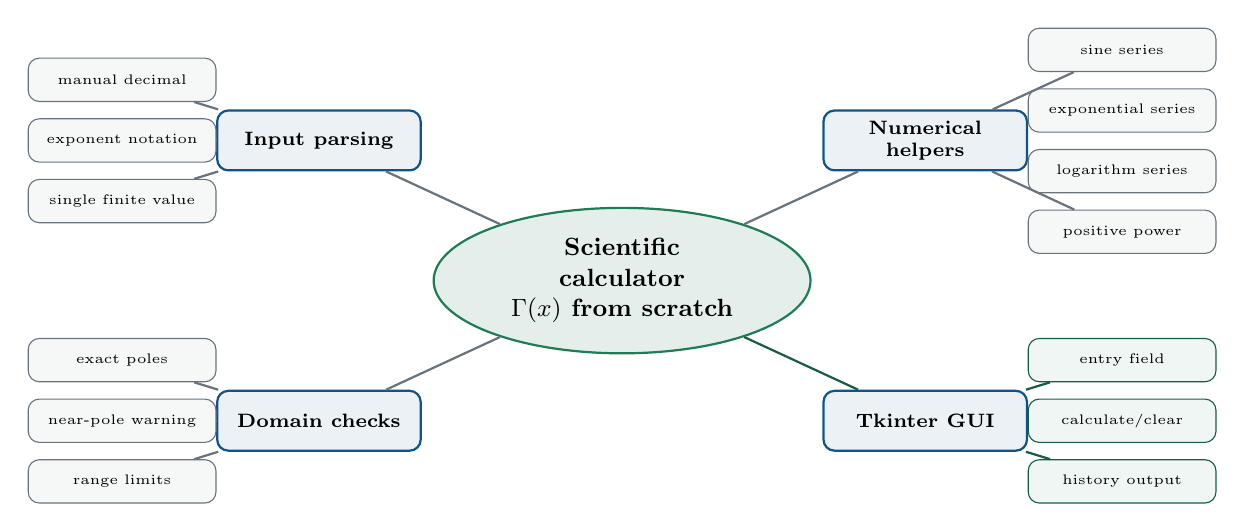
\begin{tikzpicture}[
  root/.style={ellipse,draw=softgreen,thick,fill=softgreen!12,align=center,text width=3.15cm,minimum height=1.12cm,font=\small\bfseries},
  group/.style={rectangle,rounded corners,draw=softblue,thick,fill=softblue!8,align=center,text width=2.35cm,minimum height=0.76cm,font=\scriptsize\bfseries},
  item/.style={rectangle,rounded corners,draw=linegray,fill=linegray!6,align=center,text width=2.15cm,minimum height=0.55cm,font=\tiny},
  guiitem/.style={rectangle,rounded corners,draw=softgreen!75!black,fill=softgreen!7,align=center,text width=2.15cm,minimum height=0.55cm,font=\tiny},
  branch/.style={draw=linegray,thick},
  goodbranch/.style={draw=softgreen!75!black,thick}
]
\node[root] (root) at (0,0) {Scientific calculator\\$\Gamma(x)$ from scratch};
\node[group] (parse) at (-3.85,1.78) {Input parsing};
\node[group] (domain) at (-3.85,-1.78) {Domain checks};
\node[group] (helpers) at (3.85,1.78) {Numerical helpers};
\node[group] (gui) at (3.85,-1.78) {Tkinter GUI};
\draw[branch] (root) -- (parse); \draw[branch] (root) -- (domain); \draw[branch] (root) -- (helpers); \draw[goodbranch] (root) -- (gui);
\node[item] (p1) at (-6.35,2.55) {manual decimal};
\node[item] (p2) at (-6.35,1.78) {exponent notation};
\node[item] (p3) at (-6.35,1.01) {single finite value};
\draw[branch] (parse) -- (p1); \draw[branch] (parse) -- (p2); \draw[branch] (parse) -- (p3);
\node[item] (d1) at (-6.35,-1.01) {exact poles};
\node[item] (d2) at (-6.35,-1.78) {near-pole warning};
\node[item] (d3) at (-6.35,-2.55) {range limits};
\draw[branch] (domain) -- (d1); \draw[branch] (domain) -- (d2); \draw[branch] (domain) -- (d3);
\node[item] (h1) at (6.35,2.93) {sine series};
\node[item] (h2) at (6.35,2.16) {exponential series};
\node[item] (h3) at (6.35,1.39) {logarithm series};
\node[item] (h4) at (6.35,0.62) {positive power};
\draw[branch] (helpers) -- (h1); \draw[branch] (helpers) -- (h2); \draw[branch] (helpers) -- (h3); \draw[branch] (helpers) -- (h4);
\node[guiitem] (u1) at (6.35,-1.01) {entry field};
\node[guiitem] (u2) at (6.35,-1.78) {calculate/clear};
\node[guiitem] (u3) at (6.35,-2.55) {history output};
\draw[goodbranch] (gui) -- (u1); \draw[goodbranch] (gui) -- (u2); \draw[goodbranch] (gui) -- (u3);
\end{tikzpicture}}
\vspace{0.25em}
\small
The D2 implementation decomposes $\Gamma(x)$ into input parsing, domain checks, subordinate numerical functions, and GUI behaviour instead of delegating numerical work to Python's math library.
\vfill
{\raggedright\smallnote{Sources: [2], [4].}\par}
\end{frame}

% Slide 4
\begin{frame}{P5: Tkinter GUI demonstration}
\centering
\includegraphics[width=0.93\textwidth,height=0.68\textheight,keepaspectratio]{gamma_function_result.png}
\par
\vspace{0.25em}
\scriptsize
The screenshot demonstrates the Tkinter input field, Calculate/Clear controls, calculation history, repeated use, and helpful messages for valid values, poles, invalid text, and near-pole values.
\vfill
{\raggedright\smallnote{Source: GUI execution screenshot.}\par}
\end{frame}

% Slide 5
\begin{frame}[fragile]{P5: Four-file source structure and exceptions}
\scriptsize
\begin{columns}[T,onlytextwidth]
\column{0.53\textwidth}
\begin{block}{Repository source files}
\begin{tabularx}{\linewidth}{>{\ttfamily}p{2.25cm}X}
main.py & Starts the GUI without an IDE.\\
gui.py & Tkinter widgets, events, and history.\\
gamma\_core.py & Parsing, exceptions, numerical helpers, and $\Gamma(x)$.\\
validate\_gamma.py & Validation-only reference script.\\
\end{tabularx}
\end{block}
\column{0.43\textwidth}
\begin{block}{Exception handling}
\begin{itemize}\itemsep0.2em
  \item \texttt{InputFormatError}
  \item \texttt{GammaDomainError}
  \item \texttt{GammaRangeError}
  \item \texttt{GammaUnderflowError}
\end{itemize}
Expected errors are shown in the GUI without Python tracebacks.
\end{block}
\begin{block}{Built-in review}
\texttt{range()} and \texttt{len()} are avoided in production numerical calculation; \texttt{math} is used only by \texttt{validate\_gamma.py}.
\end{block}
\end{columns}
\vfill\smallnote{Sources: [2], [5].}
\end{frame}

% Slide 6
\begin{frame}{P5: GUI behaviour and numerical validation}
\scriptsize
\begin{columns}[T,onlytextwidth]
\column{0.55\textwidth}
\begin{tabularx}{\linewidth}{p{2.2cm}X}
\toprule
Case & GUI behaviour \\
\midrule
Valid input & Shows $x$, $\Gamma(x)$, and method path. \\
Exact pole & Explains why $0,-1,-2,\ldots$ are invalid. \\
Invalid text & Asks for one finite real number. \\
Near pole & Warns that the result is numerically sensitive. \\
Overflow/underflow & Shows range-related message instead of crashing. \\
\bottomrule
\end{tabularx}
\column{0.41\textwidth}
\begin{block}{Validation policy}
\texttt{math.gamma()} is used only in a separate validation script, not in the submitted Gamma application.
\end{block}
\begin{center}
\begin{tabular}{c c}
\toprule
Cases & 8 \\
Max relative error & $1.332\times10^{-15}$ \\
Required threshold & $10^{-10}$ \\
Result & Passed \\
\bottomrule
\end{tabular}
\end{center}
\end{columns}
\vfill\smallnote{Sources: [2], [3], [5].}
\end{frame}

% Slide 7
\begin{frame}{P6: Public repository URL and contents evidence}
\scriptsize
\begin{block}{Public repository URL}
\texttt{https://github.com/arifulHossain1/soen6011-Scientific-Calculator-gamma-d2}
\end{block}

\centering

\includegraphics[width=0.94\textwidth,height=0.56\textheight,keepaspectratio]{Project github structure.PNG}
\par
\vspace{0.15em}
\scriptsize
The repository shows the required README, validation output, and the four source files:
\texttt{main.py}, \texttt{gui.py}, \texttt{gamma\_core.py}, and \texttt{validate\_gamma.py}.
\vfill
{\raggedright\smallnote{Sources: [2], [8]; actual GitHub repository screenshot.}\par}
\end{frame}

% Slide 8
\begin{frame}{P6: High-quality commit history evidence}
\centering

\includegraphics[width=0.96\textwidth,height=0.68\textheight,keepaspectratio]{Commit.PNG}
\par
\vspace{0.2em}
\scriptsize
The commit history records meaningful changes for the core calculation, GUI, IDE-independent entry point,
validation, and documentation instead of a single generic upload.
\vfill
{\raggedright\smallnote{Sources: [2], [8]; actual GitHub commit-history screenshot.}\par}
\end{frame}

% Slide 9
\begin{frame}{P7: Updated requirements summary}
\tiny
\renewcommand{\arraystretch}{1.12}
\begin{tabularx}{\textwidth}{>{\ttfamily\raggedright\arraybackslash}p{1.65cm}p{1.35cm}X p{1.7cm}}
\toprule
ID & Status & Updated direction & Verification \\
\midrule
GG-UI-01 & \statusmodified & Replace textual prompt with Tkinter entry field and buttons. & GUI inspection \\
GG-IN-01/02 & \statusmodified & Manual parsing accepts one finite real number and rejects invalid text. & Input tests \\
GG-FN-01 & \statusmodified & Compute finite real non-pole results using from-scratch Lanczos path. & Reference tests \\
GG-OU-01/02 & \statusmodified & Display result and method in GUI history. & Output test \\
GG-SE-01 & \statusmodified & Allow repeated calculations through the GUI without restarting. & Session test \\
GG-PR-01 & \statussame & Preserve $10^{-10}$ validation threshold. & Validation script \\
GG-SC-01/02 & \statusnew & Implement subordinate numerical helpers; do not call prohibited math-library routines. & Code inspection \\
GG-EX-01 & \statusnew & Handle expected errors without traceback. & Exception test \\
GG-DEP-01 & \statusnew & Run from terminal without depending on a specific IDE. & Terminal test \\
\bottomrule
\end{tabularx}
\vspace{0.45em}
\begin{block}{P7 boundary}
\scriptsize
Problem 7 updates the function and GUI requirements based on Problem 5. Repository, README, and commit-message evidence remain under Problem 6 as project constraints.
\end{block}
\vfill\smallnote{Sources: [1], [2].}
\end{frame}

\appendix

% Slide 10
\begin{frame}{Appendix: P5 -- CASTROFF Prompt Log}
\tiny
\textbf{Tool used:} ChatGPT.\\
\textbf{Prompt type:} Role-based, instructional, constraint-driven, iterative debugging.\\
\textbf{Purpose:} Support from-scratch Gamma implementation with Tkinter GUI.
\vspace{0.35em}
\begin{tabularx}{\textwidth}{>{\bfseries}p{1.45cm}X}
Constraints & Avoid production use of math-library Gamma/sin/exp/log/sqrt/pow; use Tkinter; provide helpful exceptions; review built-ins.\\
Audience & SOEN 6011 professor, TA, and students.\\
Structure & Boundary, subordinate functions, GUI behaviour, validation evidence.\\
Tone & Academic, clear, implementation-ready.\\
Role & Numerical-software developer and reviewer.\\
Output & Runnable Python source plus Beamer-ready explanation.\\
Focus & Gamma Guard GUI and from-scratch subordinate operations.\\
Function & Produce D2 P5 implementation and demonstration explanation.\\
\end{tabularx}
\begin{block}{Initial prompt used}
Modify my D1 Gamma Guard implementation for D2. It must implement Gamma from scratch in Python, use Tkinter for a GUI, avoid prohibited math-library functions in production, and provide helpful exception handling.
\end{block}
\begin{block}{Output explanation}
I accepted the modular GUI structure, then modified the implementation and slides to separate validation-only \texttt{math.gamma()}, review built-ins, and document expected errors.
\end{block}
\vfill\smallnote{Source: [6].}
\end{frame}

% Slide 11
\begin{frame}{Appendix: P6 -- CASTROFF Prompt Log}
\tiny
\textbf{Tool used:} ChatGPT.\\
\textbf{Prompt type:} Instructional, planning, documentation prompt.\\
\textbf{Purpose:} Create a repository plan, README, and high-quality commit-message examples.
\vspace{0.35em}
\begin{tabularx}{\textwidth}{>{\bfseries}p{1.45cm}X}
Constraints & Public repository, README, high-quality commits, repository URL, and screenshots of real evidence.\\
Audience & Marker reviewing D2 repository evidence.\\
Structure & Repository tree, commit sequence, README sections, evidence slides.\\
Tone & Practical and submission-ready.\\
Role & Version-control documentation assistant.\\
Output & README, .gitignore, commit plan, checklist, evidence slides.\\
Focus & Traceable Git history and clear documentation.\\
Function & Satisfy D2 P6 evidence requirements.\\
\end{tabularx}
\begin{block}{Initial prompt used}
Based on the D2 project description, tell me what to upload to GitHub, how to structure the repository, and what high-quality commit messages to use.
\end{block}
\begin{block}{Output explanation}
I kept the repository structure and commit-message guidance, but replaced planned repository claims with screenshots from the actual public repository and commit history.
\end{block}
\vfill\smallnote{Source: [6].}
\end{frame}

% Slide 12
\begin{frame}{Appendix: P7 -- CASTROFF Prompt Log}
\tiny
\textbf{Tool used:} ChatGPT.\\
\textbf{Prompt type:} Requirements-analysis, traceability, refinement prompt.\\
\textbf{Purpose:} Update D1 requirements based on the D2 GUI and from-scratch implementation.
\vspace{0.35em}
\begin{tabularx}{\textwidth}{>{\bfseries}p{1.45cm}X}
Constraints & Preserve D1 baseline; classify requirements as unchanged, modified, or new; keep repository items under P6.\\
Audience & SOEN 6011 evaluator.\\
Structure & Requirement ID, status, requirement direction, verification.\\
Tone & Formal and verifiable.\\
Role & Requirements engineer.\\
Output & Complete updated requirement list for D2.\\
Focus & Changes caused by D2 Problem 5.\\
Function & Satisfy D2 P7.\\
\end{tabularx}
\begin{block}{Initial prompt used}
Modify my D1 requirements for D2. The implementation now has a Tkinter GUI, must be from scratch, must handle exceptions, and must have helpful messages.
\end{block}
\begin{block}{Output explanation}
I used the output to produce a complete P7 requirement update, removed repository requirements from the function-requirement list, and labelled each item as unchanged, modified, or new.
\end{block}
\vfill\smallnote{Source: [6].}
\end{frame}

% Slide 13
\begin{frame}{Backup: Complete P7 requirements -- input and domain}
\tiny
\renewcommand{\arraystretch}{1.12}
\begin{tabularx}{\textwidth}{>{\ttfamily}p{1.4cm}p{1.25cm}X p{1.55cm}}
\toprule
ID & Status & Updated requirement & Verification \\
\midrule
GG-UI-01 & \statusmodified & The software shall present a Tkinter input field for one real Gamma-function argument $x$. & GUI inspection \\
GG-IN-01 & \statusmodified & When the entered text represents one finite real number, the software shall parse it using the project-defined parser. & Input test \\
GG-IN-02 & \statusmodified & When the entered text is not one finite real number, the GUI shall display a corrective input message. & Invalid-input test \\
GG-DM-01 & \statussame & When $x$ is 0 or a negative integer, the software shall display a Gamma-domain pole message. & Boundary test \\
GG-DM-02 & \statusmodified & When $x$ is within $10^{-12}$ of a nonpositive integer but is not exactly a pole, the GUI shall display a near-pole warning. & Sensitivity test \\
GG-FN-01 & \statusmodified & When $x$ is finite, not a pole, and the result is finite in double precision, the software shall compute $\Gamma(x)$ from scratch using the selected algorithm. & Reference test \\
GG-RG-01 & \statusmodified & When the Gamma value exceeds the supported range, the GUI shall display a range message. & Range test \\
GG-RG-02 & \statusmodified & When a nonzero Gamma value cannot be represented distinctly from zero, the GUI shall display an underflow message. & Underflow test \\
\bottomrule
\end{tabularx}
\vfill\smallnote{Sources: [1], [2].}
\end{frame}

% Slide 14
\begin{frame}{Backup: Complete P7 requirements -- output and quality}
\tiny
\renewcommand{\arraystretch}{1.12}
\begin{tabularx}{\textwidth}{>{\ttfamily}p{1.4cm}p{1.25cm}X p{1.55cm}}
\toprule
ID & Status & Updated requirement & Verification \\
\midrule
GG-OU-01 & \statusmodified & After a successful calculation, the GUI shall display $x$ and $\Gamma(x)$ with at least ten significant digits in the history area. & Output test \\
GG-OU-02 & \statusmodified & After a successful calculation, the GUI shall display the algorithm path used. & Output test \\
GG-SE-01 & \statusmodified & After each result or error, the GUI shall permit another calculation without restarting the application. & Session test \\
GG-PR-01 & \statussame & For the validation set $\{0.1,0.5,1,1.5,2.5,5,-0.5,-1.5\}$, relative error shall be no greater than $10^{-10}$. & Validation script \\
GG-US-01 & \statusmodified & For invalid input, domain rejection, range, or underflow, the GUI shall display a plain-language message with cause and corrective direction. & Usability test \\
\bottomrule
\end{tabularx}
\vspace{0.6em}
\begin{block}{Validation-only distinction}
\scriptsize
\texttt{math.gamma()} may be used only in \texttt{validate\_gamma.py}; it is not imported or called by the production Gamma application.
\end{block}
\vfill\smallnote{Sources: [1], [2], [5].}
\end{frame}

% Slide 15
\begin{frame}{Backup: Complete P7 requirements -- D2 additions}
\tiny
\renewcommand{\arraystretch}{1.12}
\begin{tabularx}{\textwidth}{>{\ttfamily}p{1.4cm}p{1.25cm}X p{1.55cm}}
\toprule
ID & Status & Updated requirement & Verification \\
\midrule
GG-GUI-01 & \statusnew & The software shall provide a Tkinter GUI with an input field, Calculate control, Clear control, status label, and output/history area. & GUI inspection \\
GG-SC-01 & \statusnew & The production code shall implement sine, exponential, logarithm, positive-base power, and absolute-value support as project-defined subordinate functions. & Code inspection \\
GG-SC-02 & \statusnew & The production Gamma calculation shall not call Python's math-library Gamma, sine, exponential, logarithm, square-root, or power functions. & Code inspection \\
GG-BI-01 & \statusnew & The production numerical calculation shall avoid \texttt{range()} and \texttt{len()} by using \texttt{while} loops and manual counters where needed. & Code inspection \\
GG-EX-01 & \statusnew & Expected input, domain, range, and underflow cases shall be represented by user-facing exception classes. & Exception test \\
GG-DEP-01 & \statusnew & The application shall run from a terminal command without depending on a specific IDE. & Terminal test \\
\bottomrule
\end{tabularx}
\vspace{0.45em}
\begin{block}{Separate P6 project constraints}
\scriptsize
Public repository, README, and meaningful commit messages are required project evidence for P6, not function requirements in P7.
\end{block}
\vfill\smallnote{Sources: [1], [2].}
\end{frame}

% Slide 16
\begin{frame}{Backup: Complete validation table}
\tiny
\renewcommand{\arraystretch}{1.12}
\begin{tabularx}{\textwidth}{c r r r c}
\toprule
$x$ & Gamma Guard result & Validation reference & Relative error & Status \\
\midrule
$0.1$ & $9.51350769866873$ & $9.51350769866873$ & $1.867\times10^{-16}$ & Pass \\
$0.5$ & $1.77245385090552$ & $1.77245385090552$ & $3.758\times10^{-16}$ & Pass \\
$1$ & $1$ & $1$ & $0$ & Pass \\
$1.5$ & $0.886226925452758$ & $0.886226925452758$ & $3.758\times10^{-16}$ & Pass \\
$2.5$ & $1.32934038817914$ & $1.32934038817914$ & $3.341\times10^{-16}$ & Pass \\
$5$ & $24$ & $24$ & $1.332\times10^{-15}$ & Pass \\
$-0.5$ & $-3.54490770181103$ & $-3.54490770181103$ & $7.517\times10^{-16}$ & Pass \\
$-1.5$ & $2.36327180120735$ & $2.36327180120735$ & $7.517\times10^{-16}$ & Pass \\
\bottomrule
\end{tabularx}
\vspace{0.5em}
\begin{block}{Reference policy}
\texttt{math.gamma()} is used only in the validation script. It is not called by the Gamma Guard implementation.
\end{block}
\vfill\smallnote{Sources: [3], [5].}
\end{frame}

% Slide 17
\begin{frame}{References}
\tiny
[1] D1: Gamma Guard, F4: $\Gamma(x)$, Md. Ariful Hossain, SOEN 6011, 2026.\\[0.35em]
[2] SOEN 6011, ``Project Description,'' Concordia University, Summer 2026.\\[0.35em]
[3] NIST Digital Library of Mathematical Functions, ``Gamma Function,'' ch. 5. [Online]. Available: \texttt{https://dlmf.nist.gov/5}.\\[0.35em]
[4] R. Munafo, ``Coefficients for the Lanczos Approximation to the Gamma Function,'' 2019. [Online]. Available: \texttt{https://www.mrob.com/pub/ries/lanczos-gamma.html}.\\[0.35em]
[5] Python Software Foundation, ``math -- Mathematical functions,'' Python documentation. [Online]. Available: \texttt{https://docs.python.org/3/library/math.html}.\\[0.35em]
[6] H. Tavakoli, \emph{Prompt Engineering for Everyone: A Self-Taught, Human-Centered Approach to AI Programming}. Berkeley, CA, USA: Apress, 2026.\\[0.35em]
[7] Python Software Foundation, ``tkinter -- Python interface to Tcl/Tk,'' Python documentation. [Online]. Available: \texttt{https://docs.python.org/3/library/tkinter.html}.\\[0.35em]
[8] GitHub Docs, ``About READMEs'' and ``About commits,'' GitHub documentation. [Online]. Available: \texttt{https://docs.github.com/}.
\end{frame}

\end{document}
